%\hypertarget{___gatsby}{}
%\hypertarget{gatsby-focus-wrapper}{}
%\href{https://mukulrathi.com/}{}
%
%MUKUL RATHI
%
%\href{https://mukulrathi.com/about-me}{}
%
%About Me
%
%\href{https://mukulrathi.com/blog}{}
%
%Blog
%
%\hypertarget{creating-the-bolt-compiler-part-3}{%
%\subsection{Creating the Bolt Compiler: Part
%3}\label{creating-the-bolt-compiler-part-3}}

\hypertarget{top-of-page}{%
\chapter{Writing a Lexer and Parser using OCamllex and
Menhir}\label{top-of-page}}

June 01, 2020

%\hypertarget{min-read}{%
%\subsection{10 min read}\label{min-read}}
%
%\hypertarget{last-updated-february-05-2022}{%
%\subsection{Last updated: February 05,
%2022}\label{last-updated-february-05-2022}}

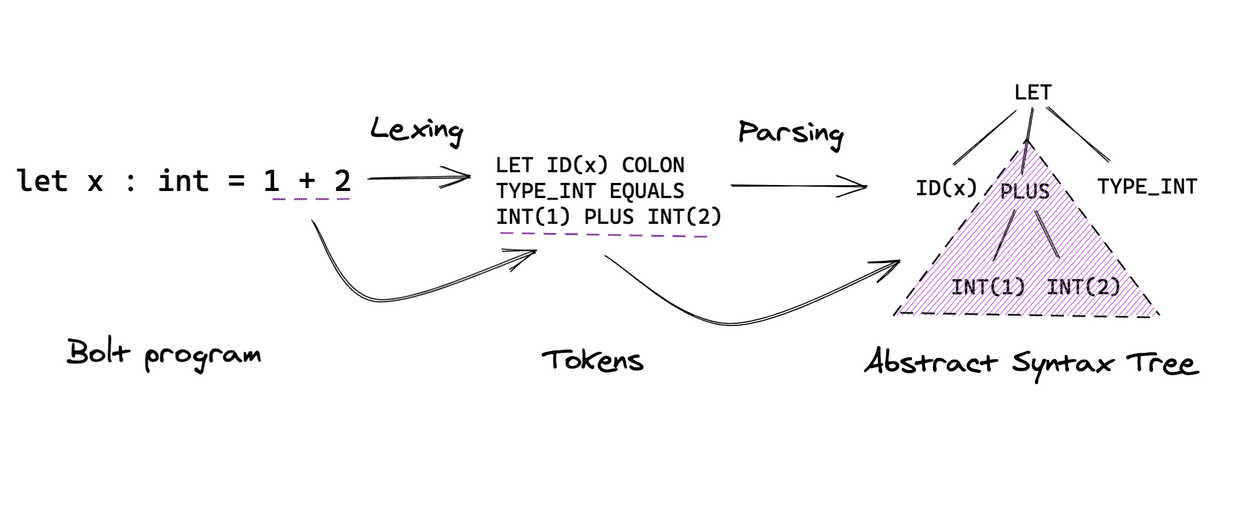
\includegraphics[width=\linewidth]{03_files/parsing-overview.png}

%\hypertarget{series-creating-the-bolt-compiler}{%
%\section{Series: Creating the Bolt
%Compiler}\label{series-creating-the-bolt-compiler}}
%
%\begin{itemize}
%\item
%  { Part 1:
%  }\href{https://mukulrathi.com/create-your-own-programming-language/intro-to-compiler/}{How
%  I wrote my own "proper" programming language}
%\item
%  { Part 2:
%  }\href{https://mukulrathi.com/create-your-own-programming-language/compiler-engineering-structure/}{So
%  how do you structure a compiler project?}
%\item
%  \textbf{Part 3: Writing a Lexer and Parser using OCamllex and Menhir}
%\item
%  { Part 4:
%  }\href{https://mukulrathi.com/create-your-own-programming-language/intro-to-type-checking/}{An
%  accessible introduction to type theory and implementing a
%  type-checker}
%\item
%  { Part 5:
%  }\href{https://mukulrathi.com/create-your-own-programming-language/data-race-dataflow-analysis/}{A
%  tutorial on liveness and alias dataflow analysis}
%\item
%  { Part 6:
%  }\href{https://mukulrathi.com/create-your-own-programming-language/lower-language-constructs-to-llvm/}{Desugaring
%  - taking our high-level language and simplifying it!}
%\item
%  { Part 7:
%  }\href{https://mukulrathi.com/create-your-own-programming-language/protobuf-ocaml-cpp-tutorial/}{A
%  Protobuf tutorial for OCaml and C++}
%\item
%  { Part 8:
%  }\href{https://mukulrathi.com/create-your-own-programming-language/llvm-ir-cpp-api-tutorial/}{A
%  Complete Guide to LLVM for Programming Language Creators}
%\item
%  { Part 9:
%  }\href{https://mukulrathi.com/create-your-own-programming-language/concurrency-runtime-language-tutorial/}{Implementing
%  Concurrency and our Runtime Library}
%\item
%  { Part 10:
%  }\href{https://mukulrathi.com/create-your-own-programming-language/generics-parametric-polymorphism/}{Generics
%  - adding polymorphism to Bolt}
%\item
%  { Part 11:
%  }\href{https://mukulrathi.com/create-your-own-programming-language/inheritance-method-overriding-vtable/}{Adding
%  Inheritance and Method Overriding to Our Language}
%\end{itemize}
%
%\begin{center}\rule{0.5\linewidth}{0.5pt}\end{center}

We can't directly reason about our Bolt program, as it is just an
unstructured stream of characters. Lexing and parsing
\emph{pre-processes} them into a structured representation that we can
perform type-checking on in later stages of the compiler.

\hypertarget{lexing-tokens}{%
\section{\texorpdfstring{\protect\hyperlink{lexing-tokens}{}Lexing
Tokens}{Lexing Tokens}}\label{lexing-tokens}}

The individual characters don't mean much, so first we need to split the
stream into \emph{tokens} (which are analogous to ``words'' in
sentences). These tokens assign meaning: is this group of characters a
specific keyword in our language (\texttt{if} \texttt{int}
\texttt{class}) or is it an identifier (\texttt{banana})?

Tokens also reduce our problem space substantially: they standardise the
representation. We no longer have to worry about whitespace
(\texttt{x\ ==\ 0} and \texttt{x==\ 0} both become
\texttt{IDENTIFIER(x)\ EQUAL\ EQUAL\ INT(0)}) and we can filter out
comments from our source code.

How do we split our stream of characters into tokens? We
\emph{pattern-match}. Under the hood, you could think of this as a
massive case analysis. However, since the case analysis is ambiguous
(multiple tokens could correspond to the same set of characters) we have
two additional rules we have to consider:

\begin{enumerate}
\tightlist
\item
  \textbf{Priority order:} We order our tokens by priority. E.g. we want
  \texttt{int} to be matched as a keyword, not a variable name.
\item
  \textbf{Longest pattern match:} we read \texttt{else} as a keyword
  rather than splitting it into two variable names \texttt{el} and
  \texttt{se}. Likewise, \texttt{intMax} is a variable name: not to be
  read as \texttt{int} and \texttt{Max}.
\end{enumerate}

Here's a really simple lexer that recognises the keywords ``IN'',
``INT'' and identifiers (variable / function names), and tokens are
separating by spaces. Notice we check for the IN case before the
``default'' variable case (priority order):

Copy

\begin{verbatim}
// this is pseudocode for a simplified lexerchars
SeenSoFar = "in"while(streamHasMoreCharacters){  nextChar = readCharFromStream()  if(nextChar == " "){      // we've found a token      switch(charsSeenSoFar):        case "in":          output "IN"          break      case: "int":        output "INT"        break      default:        output ID(charsSeenSoFar)        // not "in" or "int" keywords so must be an identifier      charSeenSoFar= ""  // start matching another token  } else {    // longest match: we'll try to pattern match "int" next iteration    charSeenSoFar += nextChar  }}
\end{verbatim}

\hypertarget{ocamllex}{%
\section{\texorpdfstring{\protect\hyperlink{ocamllex}{}OCamllex}{OCamllex}}\label{ocamllex}}

Whilst you could hand-code the pattern-matching pseudocode, in practice
it is quite finicky especially as our language gets bigger. Instead,
we're going to use the lexer generator \textbf{OCamllex}. OCamllex is an
OCaml library we can use in our compiler by adding it as a dependency to
our Dune build file.

%{
%\href{https://github.com/mukul-rathi/bolt/blob/master/src/frontend/parsing/dune\#L10}{dune}}
%
%Copy

\begin{verbatim}
(ocamllex lexer)
\end{verbatim}

The specification for the lexer is in the \texttt{lexer.mll} file (note
the \texttt{.mll} file extension).

\hypertarget{ocaml-header}{%
\subsection{\texorpdfstring{\protect\hyperlink{ocaml-header}{}OCaml
Header}{OCaml Header}}\label{ocaml-header}}

To start with, we optionally provide a header containing OCaml helper
code (enclosed in curly braces). We define a \texttt{SyntaxError}
exception and a function \texttt{nextline}, which moves the pointer to
the next line of the \texttt{lexbuf} buffer that the program is read
into:

%{
%\href{https://github.com/mukul-rathi/bolt/blob/master/src/frontend/parsing/lexer.mll}{lexer.mll}}
%
%Copy

\begin{lstlisting}[language=caml,caption={{lexer.mll}}]
{open Lexingopen Parser
exception SyntaxError of string
let next_line lexbuf =  let pos = lexbuf.lex_curr_p in  lexbuf.lex_curr_p <-    { pos with pos_bol = lexbuf.lex_curr_pos;               pos_lnum = pos.pos_lnum + 1    }}
\end{lstlisting}

\hypertarget{helper-regexes}{%
\subsection{\texorpdfstring{\protect\hyperlink{helper-regexes}{}Helper
Regexes}{Helper Regexes}}\label{helper-regexes}}

Next, we need to specify the regular expressions we're using to match
the tokens. For most of the tokens, this is a simple string e.g.
\texttt{true} for token \texttt{TRUE}. However, other tokens have more
complex regexes e.g. for integers and identifiers (below).
\href{https://caml.inria.fr/pub/docs/manual-ocaml/lexyacc.html\#ss:ocamllex-regexp}{OCamllex's
regex syntax} is like most regex libraries;
%
%{
%\href{https://github.com/mukul-rathi/bolt/blob/master/src/frontend/parsing/lexer.mll}{lexer.mll}}


\begin{lstlisting}[language=caml,caption={{lexer.mll}}]
(* Define helper regexes *)
let digit = ['0'-'9']let alpha = ['a'-'z' 'A'-'Z']
let int = '-'? digit+  (* regex for integers *)
let id = (alpha) (alpha|digit|'_')* 
(* regex for identifier *)
let whitespace = [' ' '\t']+
let newline = '\r' | '\n' | "\r\n"
\end{lstlisting}

\hypertarget{lexing-rules}{%
\subsection{\texorpdfstring{\protect\hyperlink{lexing-rules}{}Lexing
Rules}{Lexing Rules}}\label{lexing-rules}}

Next, we need to specify rules for OCamllex to scan the input. Each rule
is specified in a pattern-matching format, and we specify the regexes in
order of priority (highest priority first):


\begin{verbatim}
rule <rule_name> = parse | <regex>  {  TOKEN_NAME } (* output a token *)
                   | <regex>  { ... } (* or execute other code *)
and <another_rule> = parse  | ...
\end{verbatim}

The rules are recursive: once it matches a token, it calls itself to
start over and match the next token. Multiple rules are \emph{mutually
recursive}, that is we can recursively call each rule in the other's
definition. Having multiple rules is useful if you want to treat the
character stream differently in different cases.

For example, we want our main rule to read tokens. However, we want to
treat comments differently, not emitting any tokens until we reach the
end of the comment. Another case are strings in Bolt: we want to treat
the characters we are reading as part of a string, not as matching a
token. These cases can all be seen in the following Bolt code:

{example.bolt}

\begin{verbatim}
let x = 4 // here is a comment
/* This is a multi-line   
comment*/
printf("x's value is %d", x)
\end{verbatim}

Now we have our requirements for our lexer, we can define the rules in
our OCamllex specification file. The key points are:

\begin{itemize}
\tightlist
\item
  We have 4 rules: \texttt{read\_token},
  \texttt{read\_single\_line\_comment},
  \texttt{read\_multi\_line\_comment} and \texttt{read\_string}.
\item
  We need to handle \texttt{eof} explicitly (this signifies the end of
  file) and include a catch-all case \texttt{\_} to match all other
  regexes.
\item
  We use \texttt{Lexing.lexeme\ lexbuf} to get the string matched by the
  regex.
\item
  For \texttt{read\_string}, we create another buffer to store the
  characters into: we don't use \texttt{Lexing.lexeme\ lexbuf} as we
  want to explicitly handle escaped characters.
  \texttt{Buffer.create\ 17} allocates a resizable buffer that initially
  has a size of 17 bytes.
\item
  We use \texttt{raise\ SyntaxError} for error-handling (unexpected
  input characters).
\item
  When reading tokens, we skip over whitespace by calling
  \texttt{read\_token\ lexbuf} rather than emitting a token. Likewise,
  for a new line we call our helper function \texttt{next\_line} to skip
  over the new line character.
\end{itemize}

%{
%\href{https://github.com/mukul-rathi/bolt/blob/master/src/frontend/parsing/lexer.mll}{lexer.mll}}


\begin{lstlisting}[caption={{lexer.mll}}]
rule read_token =  parse  
                | "(" { LPAREN }  ... (* keywords and other characters' regexes *)  
                | "printf" {PRINTF }  
                | whitespace { read_token lexbuf }  
                | "//" { single_line_comment lexbuf (* use our comment rule for rest of line *) } 
                | "/*" { multi_line_comment lexbuf }  
                | int { INT (int_of_string (Lexing.lexeme lexbuf))}  
                | id { ID (Lexing.lexeme lexbuf) }    
                | '"'      { read_string (Buffer.create 17) lexbuf }  
                | newline { next_line lexbuf; read_token lexbuf }  
                | eof { EOF }  
                | _ {raise (SyntaxError ("Lexer - Illegal character: " ^ Lexing.lexeme lexbuf)) }
and read_single_line_comment = parse  
                             | newline { next_line lexbuf; read_token lexbuf }  
                             | eof { EOF }  
                             | _ { read_single_line_comment lexbuf }
and read_multi_line_comment = parse  
                            | "*/" { read_token lexbuf }  
                            | newline { next_line lexbuf; read_multi_line_comment lexbuf }  
                            | eof { raise (SyntaxError ("Lexer - Unexpected EOF - please terminate your comment.")) }  
                            | _ { read_multi_line_comment lexbuf }
and read_string buf = parse  
                    | '"'       { STRING (Buffer.contents buf) }  
                    | '\\' 'n'  { Buffer.add_char buf '\n'; read_string buf lexbuf }  
                      ... (* Other regexes to handle escaping special characters *)  
                    | [^ '"' '\\']+    { Buffer.add_string buf (Lexing.lexeme lexbuf);      
                                         read_string buf lexbuf    }  
                    | _ { raise (SyntaxError ("Illegal string character: " ^ Lexing.lexeme lexbuf)) }  
                    | eof { raise (SyntaxError ("String is not terminated")) }
\end{lstlisting}

\hypertarget{generated-ocamllex-output}{%
\subsection{\texorpdfstring{\protect\hyperlink{generated-ocamllex-output}{}Generated
OCamllex
output}{Generated OCamllex output}}\label{generated-ocamllex-output}}

OCamllex generates a \texttt{Lexer} module from the \texttt{lexer.mll}
specification, from which you can call \texttt{Lexer.read\_token} or any
of the other rules, as well as the helper functions defined in the
header. If you're curious, after running \texttt{make\ build} you can
see the generated module in \texttt{lexer.ml} in the \texttt{\_build}
folder - it's just a massive pattern-match statement:




\begin{lstlisting}[language=caml,caption={{\_build/..../lexer.ml}}]
let rec read_token lexbuf =   __ocaml_lex_read_token_rec lexbuf 0and __ocaml_lex_read_token_rec lexbuf __ocaml_lex_state =  match Lexing.engine __ocaml_lex_tables __ocaml_lex_state lexbuf  with| 0 -># 39 "src/frontend/parsing/lexer.mll"        ( LPAREN )# 2603 "src/frontend/parsing/lexer.ml"
  | 1 -># 40 "src/frontend/parsing/lexer.mll"        ( RPAREN )# 2608 "src/frontend/parsing/lexer.ml"
  | 2 -># 41 "src/frontend/parsing/lexer.mll"        ( LBRACE )# 2613 "src/frontend/parsing/lexer.ml"
  | 3 -># 42 "src/frontend/parsing/lexer.mll"        ( RBRACE )# 2618 "src/frontend/parsing/lexer.ml"
  | 4 -># 43 "src/frontend/parsing/lexer.mll"        ( COMMA )# 2623 "src/frontend/parsing/lexer.ml"
\end{lstlisting}

\hypertarget{grammar}{%
\section{\texorpdfstring{\protect\hyperlink{grammar}{}Grammar}{Grammar}}\label{grammar}}

We use structure to reason about sentences - even if we don't think
about it. The words on their own don't tell us much about the sentence -
``use'' is both a noun and verb - it's only because we have a
subject-verb-object pattern in ``we use structure'' can we infer that
``use'' is a verb. The same is true for compilers: The individual tokens
\texttt{x}, \texttt{+}, \texttt{y} don't mean much, but we can infer
from \texttt{x+y} that \texttt{x} and \texttt{y} are numbers being added
together.

We specify the structure of programs in Bolt using a \emph{grammar},
which consists of a set of rules (\emph{productions}) about how we can
construct Bolt expressions.

For example, a program consists of a list of class definitions,
following by some function definitions following by the main expression.
This would look like this (using ``X\_defns'' plural to informally refer
to a list of ``X\_defn'' ).

\textbf{program {{{\(:: =\)}{{{}{::=}}}}} class\_defns function\_defns
main\_expr}

This top level rule also has rules for each of the expressions on the
right hand side. Expressions that can be expanded further with rules are
called \emph{non-terminals}, and those that can't i.e. the tokens are
called \emph{terminals}. Let's look at the \textbf{class\_defn} rule and
\textbf{main\_expr} rules.

A class definition consists of a \texttt{CLASS} keyword token (tokens
are in UPPERCASE) followed by an \texttt{ID} token (identifier = the
class name) and then the body is enclosed by braces. The body consists
of capability definitions (this is Bolt-specific - used to prevent data
races), field definitions and then method definitions. Here the
\texttt{CLASS}, \texttt{ID}, \texttt{LBRACE} and \texttt{RBRACE} tokens
are \emph{terminals}, and the \texttt{capability\_defn},
\texttt{field\_defns} and \texttt{method\_defns} expressions are
\emph{non-terminals} (they have their own rules expanding them).

\textbf{class\_defn {{{\(:: =\)}{{{}{::=}}}}} CLASS ID LBRACE
capability\_defn field\_defns method\_defns RBRACE}

A class definition that satisfies the rules:



%Copy

\begin{lstlisting}[caption={{class\_example.bolt}}]
class Foo { 
    // Foo is the identifier  
    capability linear Bar; // capability definition (has its own rule)  
    // field defns  
    var int f : Bar; 
    // (field has Bolt-specific capability annotatation)  
    const bool g : Bar;  
    //method defns  
    int getF() : Bar {  
       // method definition (again has its own rule)    this.f  
    }
}
\end{lstlisting}

And our main expression has the following rule:

\textbf{main\_expr {{{\(:: =\)}{{{}{::=}}}}} TYPE\_VOID MAIN LPAREN
RPAREN block\_expr}

%{main\_example.bolt}
%
%Copy

\begin{verbatim}
void main() {  ...}
\end{verbatim}

Expressions can have multiple forms:

\textbf{expr {{{\(:: =\)}{{{}{::=}}}}}}

\textbf{\textbar{} NEW ID LPAREN constructor\_args RPAREN}

\textbf{\textbar{} IF expr block\_expr ELSE block\_expr}

\textbf{\textbar{} LET ID EQUAL expr}

and so on.

Full details of Bolt's grammar are in
\href{https://github.com/mukul-rathi/bolt-dissertation/blob/master/dissertation.pdf}{the
appendix of my dissertation}.

\hypertarget{abstract-syntax-trees}{%
\section{\texorpdfstring{\protect\hyperlink{abstract-syntax-trees}{}Abstract
Syntax Trees}{Abstract Syntax Trees}}\label{abstract-syntax-trees}}

If we look at this grammar from another angle, this actually specifies a
hierarchy on our program structure. At the top-level you have our
\textbf{program} rule, and then we recursively expand out each of the
terms on the right-hand-side of the rule (e.g. expand out the class
definition using its rule, main expression using its rule etc.) until we
end up with the tokens.

Which data structure represents hierarchies? \emph{Trees}. So the
grammar also specifies a \emph{syntax tree} for our Bolt program, where
tokens are the leaves.

We could display all tokens on our tree (this would be a \emph{concrete
syntax tree}) but in practice not all tokens are useful. For example, in
the expression \texttt{let\ x\ :\ int\ =\ 1+2}, you care about the
\texttt{ID} token (variable \texttt{x}) and the expression \texttt{1+2}
being assigned to the variable. We don't need to represent the
\texttt{=} token in our tree, as it doesn't convey additional meaning
(we already know we're declaring a variable). By removing these
unnecessary tokens, we end up with an \emph{abstract syntax tree} (AST).

{
\href{https://mukulrathi.com/static/60bd02e28678a6745cea6186af1f8d1b/0da74/concrete-vs-ast.png}{{}
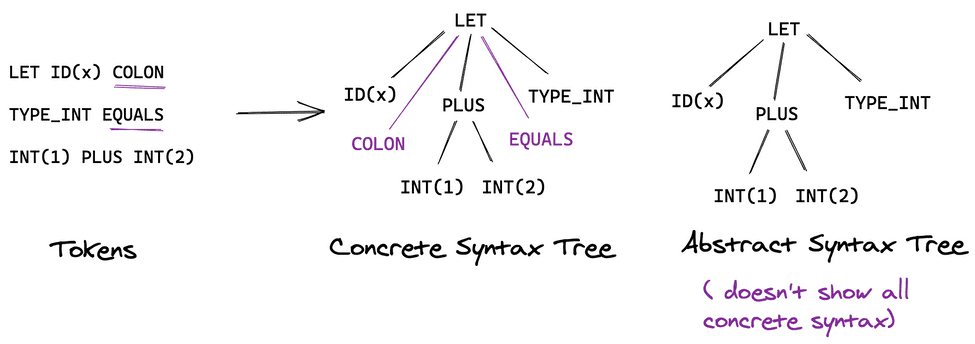
\includegraphics[width=\linewidth]{03_files/concrete-vs-ast.png}} }

The goal of parsing is to construct an Abstract Syntax Tree from a Bolt
program. The subsequent compiler stages then analyse and transform this
parsed AST to form other intermediate ASTs.

Here we split the type definitions for our AST into two files:

\texttt{ast\_types.mli} contains types common to \emph{all} ASTs across
the compiler.
%
%{
%\href{https://github.com/mukul-rathi/bolt/blob/master/src/frontend/ast/ast_types.mli}{ast\_types.mli}}
%
%Copy

\begin{lstlisting}[language=caml,caption={ast\_types.mli}]
(** Stores the line and position of the token *)
type loc = Lexing.position
type bin_op =  | BinOpPlus  | BinOpMinus  | BinOpNotEq
type modifier = MConst  (** Immutable *) 
              | MVar  (** Mutable *)
(** An abstract type for identifiers *)
module type ID = sig  type t
  val of_string : string -> t  
  val to_string : t -> string  
  val ( = ) : t -> t -> boolend
module Var_name : ID
module Class_name : ID
(** Define types of expressions in Bolt programs*)
type type_expr =  | TEInt  | TEClass   of Class_name.t  | TEVoid  | TEBool
  ...
\end{lstlisting}

\texttt{parsed\_ast.mli} contains the OCaml variant types for the class
definitions, function defns and expressions, which are essentially a
mapping of the grammar rules.

%{
%\href{https://github.com/mukul-rathi/bolt/blob/master/src/frontend/parsing/parsed_ast.mli}{parsed\_ast.mli}}
%
%Copy

\begin{lstlisting}[language=caml,caption={{parsed\_ast.mli}}]
type expr =  | Integer     of loc * int  ...  
             | Constructor of loc * Class_name.t * type_expr option * constructor_arg list  (* optional type-parameter *)  
             | Let         of loc * type_expr option * Var_name.t * expr  (* binds variable to expression (optional type annotation) *)  
             | Assign      of loc * identifier * expr  
             | MethodApp   of loc * Var_name.t * Method_name.t * expr list (* read as x.m(args) *)  
             | If          of loc * expr * block_expr * block_expr (* If ___ then ___ else ___ *)  
             | BinOp       of loc * bin_op * expr * expr  ...and block_expr = Block of loc * expr list
type class_defn =  | TClass of Class_name.t * capability list  * field_defn list * method_defn list...
\end{lstlisting}

Note \texttt{Class\_name.t}, \texttt{Var\_name.t} and
\texttt{Method\_name.t} used rather than just a string as these types
give us more information.

\hypertarget{menhir}{%
\section{\texorpdfstring{\protect\hyperlink{menhir}{}Menhir}{Menhir}}\label{menhir}}

As with lexing, we \emph{could} code this up by hand, but it would again
get a lot more finicky as our language scales. We're going to use the
parser generator \textbf{Menhir}. Again as with the lexer, we have a
\texttt{parser.mly} (note \texttt{.mly} extension) specification file.

We need to add Menhir to the Dune build file.

%{
%\href{https://github.com/mukul-rathi/bolt/blob/master/src/frontend/parsing/dune\#L12:L13}{dune}}


\begin{verbatim}
(menhir (modules parser))
\end{verbatim}

Unlike with OCamllex, we also need to update our main Dune project build
file to use Menhir:

%{
%\href{https://github.com/mukul-rathi/bolt/blob/master/dune-project\#L3}{dune-project}}


\begin{lstlisting}[caption={dune-project}]
(using menhir 2.0)
\end{lstlisting}

OCamllex and Menhir have a lot of parallels. We start with our optional
OCaml header (here this just ignores the autogenerated parser file when
calculating test coverage and opens the \texttt{Ast\_types} and
\texttt{Parsed\_ast} modules):

%{
%\href{https://github.com/mukul-rathi/bolt/blob/master/src/frontend/parsing/parser.mly}{parser.mly}}
%

\begin{lstlisting}[caption={parser.mly}]
%{
  [@@@coverage exclude_file]
  open Ast.Ast_types
  open Parsed_ast
%}
\end{lstlisting}

We then specify the tokens we'd defined in OCamllex (OCamllex and Menhir
work seamlessly together):

%{
%\href{https://github.com/mukul-rathi/bolt/blob/master/src/frontend/parsing/parser.mly}{parser.mly}}


\begin{lstlisting}[caption={parser.mly}]
%token  <int> INT
%token  <string> ID
%token  LPAREN
%token  RPAREN...
\end{lstlisting}

\hypertarget{specifying-production-signatures}{%
\subsection{\texorpdfstring{\protect\hyperlink{specifying-production-signatures}{}Specifying
Production
Signatures}{Specifying Production Signatures}}\label{specifying-production-signatures}}

Next, we specify the name of the top-level grammar production (here it
is \texttt{program}):

%{
%\href{https://github.com/mukul-rathi/bolt/blob/master/src/frontend/parsing/parser.mly}{parser.mly}}
%

\begin{lstlisting}[caption={{parser.mly}}]
%start program
\end{lstlisting}

We mentioned earlier that there was a mapping between OCaml variant
types and the grammar productions, now we specify this, so Menhir knows
what type to output when it generates the parser. This is done as a
series of
\texttt{\%type\ \textless{}ast\_type\textgreater{}\ production\_name}:

%{
%\href{https://github.com/mukul-rathi/bolt/blob/master/src/frontend/parsing/parser.mly}{parser.mly}}
%

\begin{lstlisting}[caption={{parser.mly}}]
%type <Parsed_ast.program> program
/* Class defn types */
%type <class_defn> class_defn...
%type <Capability_name.t list> class_capability_annotations
\end{lstlisting}

Note, since we opened the \texttt{Ast\_types} and \texttt{Parsed\_ast}
modules in the header, we can write \texttt{Capability\_name.t} rather
than \texttt{Ast.Ast\_types.Capability\_name.t} and \texttt{class\_defn}
instead of \texttt{Parsed\_ast.class\_defn}. However, we need to specify
absolute types for the top-level production
(\texttt{Parsed\_ast.program} not just \texttt{program}) since this
production is exposed in the \texttt{parser.mli} interface:

\begin{lstlisting}[language=caml,caption={parser.mli}]
(* this file is autogenerated by Menhir *)val program: (Lexing.lexbuf -> token) -> Lexing.lexbuf -> (Parsed_ast.program)
(* if we used program not Parsed_ast.program *)val program: (Lexing.lexbuf -> token) -> Lexing.lexbuf -> (program)(* now parser.mli doesn't know where to find program's type definition *)
\end{lstlisting}

\hypertarget{grammar-rules}{%
\subsection{\texorpdfstring{\protect\hyperlink{grammar-rules}{}Grammar
Rules}{Grammar Rules}}\label{grammar-rules}}

Finally, we can specify our grammar rules, with the returned OCaml
variant expression in \texttt{\{\}} after the rule. We can optionally
separate each of the non-terminal/terminals that make up the
right-hand-side of the rule with semicolons for readability. To use the
result of an expanded non-terminal (e.g. the \texttt{class\_defn}) in
the OCaml expression, we can refer to it with a variable
\texttt{class\_defns} (in general the form is
\texttt{var\_name}=\texttt{nonterminal\ expression}).

%{
%\href{https://github.com/mukul-rathi/bolt/blob/master/src/frontend/parsing/parser.mly}{parser.mly}}
%
%Copy

\begin{lstlisting}[caption={parser.mly}]
program:| class_defns=list(class_defn); function_defns=list(function_defn); main= main_expr;  EOF {Prog(class_defns, function_defns, main)}
\end{lstlisting}

Menhir provides a lot of small helper functions that make writing the
parser easier. We've seen \texttt{list(class\_defn)} - this returns the
type \texttt{Parsed\_ast.class\_defn\ list}. There are other variants of
this e.g. \texttt{separated\_list()} and \texttt{nonempty\_list()} and
\texttt{separated\_nonempty\_list()}:

%{
%\href{https://github.com/mukul-rathi/bolt/blob/master/src/frontend/parsing/parser.mly}{parser.mly}}
%
%Copy

\begin{lstlisting}[caption={parser.mly}]
params:| LPAREN; params=separated_list(COMMA,param); RPAREN {params}
param_capability_annotations:| LBRACE;  capability_names=separated_nonempty_list(COMMA,capability_name); RBRACE {capability_names}
\end{lstlisting}

Another useful function is \texttt{option()}. Here since
\texttt{let\_type\_annot} returns an OCaml expression of type
\texttt{Parsed\_ast.type\_expr}, \texttt{option(let\_type\_annot)}
returns a value of type \texttt{Parsed\_ast.type\_expr\ option} - this
is useful for cases where the user might optionally add type
annotations. e.g. \texttt{let\ x\ :\ int\ =\ 5} vs
\texttt{let\ x\ =\ 5}.

Finally, Menhir also lets us get the line number and position of the
production in the program (we'd defined the type \texttt{loc} for this),
which is useful for error messages! You can decide from where to get the
position: I chose to get the position at the start of the production
using \texttt{\$startpos}.

%{
%\href{https://github.com/mukul-rathi/bolt/blob/master/src/frontend/parsing/parser.mly}{parser.mly}}
%
%Copy

\begin{lstlisting}
expr:| i=INT {Integer($startpos, i)}
     | TRUE { Boolean($startpos, true)}
     | FALSE {  Boolean($startpos, false) }...+
     | e1=expr op=bin_op e2=expr {BinOp($startpos, op, e1, e2)}
     | LET; var_name=ID; type_annot=option(let_type_annot);  EQUAL; bound_expr=expr  {Let($startpos, type_annot, Var_name.of_string var_name, bound_expr)}
     | id=identifier; COLONEQ; assigned_expr=expr {Assign($startpos, id, assigned_expr)}
\end{lstlisting}

\hypertarget{resolving-ambiguous-parses}{%
\subsection{\texorpdfstring{\protect\hyperlink{resolving-ambiguous-parses}{}Resolving
ambiguous
parses}{Resolving ambiguous parses}}\label{resolving-ambiguous-parses}}

Sometimes our grammar can produce \emph{multiple} abstract syntax trees,
in which case we say it is \emph{ambiguous}. The classic example is if
we have the following grammar:

\textbf{expr {{{\(:: =\)}{{{}{::=}}}}} \textbar{} INT \textbar{} expr
PLUS expr \textbar{} expr MULT expr}

{
\href{https://mukulrathi.com/static/23049100e53e9ffd7b0c6afc4e8a1bfd/bf8c1/ambig-parse.png}{{}
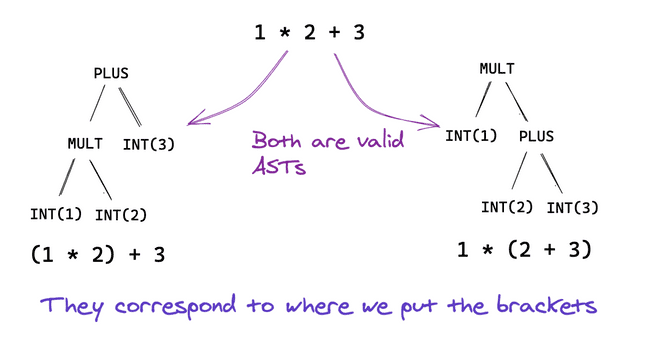
\includegraphics[width=\linewidth]{03_files/ambig-parse.png}} }

If we try to build this grammar with Menhir, then we get the following
error message (the numbers aren't important, Bolt has many more
operators than just + and - ):

%Copy

\begin{verbatim}
menhir src/frontend/parsing/parser.{ml,mli}
Warning: 17 states have shift/reduce conflicts.
Warning: 187 shift/reduce conflicts were arbitrarily resolved.
\end{verbatim}

Arbitrarily resolved isn't good! This means it'll randomly pick one,
even if it's not the one we want. To fix this we have two options

\begin{enumerate}
\tightlist
\item
  Rewrite the grammar to be unambiguous.
\item
  Keep the ambiguity but tell Menhir how to resolve it.
\end{enumerate}

I had initially chosen option 1 for Bolt. It is possible to do this for
\href{https://stackoverflow.com/a/3106287/6752788}{small grammars} but
this becomes harder as your language gets bigger. The main disadvantage
is that you have to put extra parentheses around Bolt expressions to
disambiguate parses, which really isn't a good experience.

When writing this post, I looked at the OCaml compiler for inspiration
(it too uses Menhir!) and the Menhir docs. Option 2 offers a better
solution, but first we need to understand how Menhir works.

Menhir is a \emph{shift-reduce} parser. It builds our AST bottom-up,
deciding based on the next token whether to \emph{reduce} the current
stack of non-terminals and terminals (i.e. it matches the
right-hand-side of a production rule, so reduce it to the
left-hand-side) or to \emph{shift} another token onto the stack.

{
\href{https://mukulrathi.com/static/e2c460bd0a6bcc3f1ab33fc4f962c906/2215f/shift-reduce-parser.png}{{}
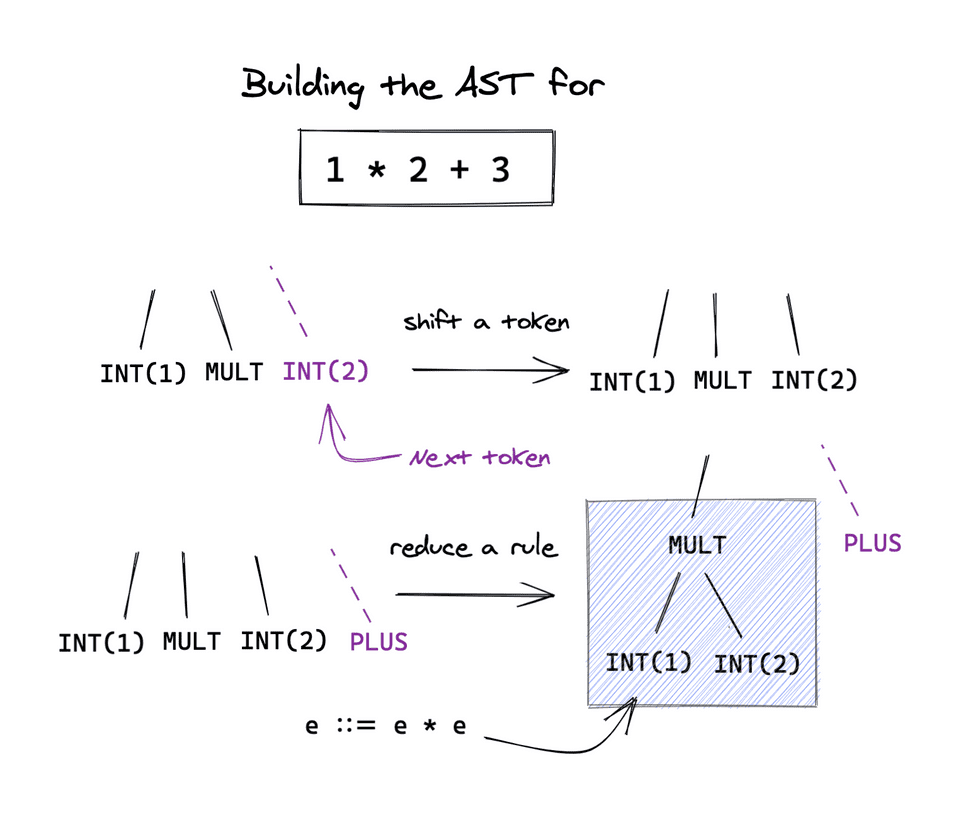
\includegraphics[width=\linewidth]{03_files/shift-reduce-parser.png}} }

A \emph{shift-reduce conflict} occurs when it could do both and end up
with a valid AST in either case. Menhir lets us manually specify which
action to take in the form
\texttt{\textless{}action\textgreater{}\ token} whether the action is:

\begin{enumerate}
\tightlist
\item
  \texttt{\%left}: reduce
\item
  \texttt{\%right}: shift
\item
  \texttt{\%nonassoc}: raise a SyntaxError
\end{enumerate}

If you're not sure which one to choose, you have a secret weapon!

Running \texttt{menhir\ src/frontend/parsing/parser.mly\ -\/-explain}
will generate an explanation in a \texttt{parser.conflicts} file, which
gives an in-depth explanation as to where the conflict is!

This is only part of the story - we want to specify that multiplication
takes precedence over addition. We can do this by specifying an
\emph{ordering} on the actions, from lowest priority to highest. Then
when there are multiple rules, Menhir will choose the one with the
highest priority - it will reduce the multiplication before the addition
in our example, giving us the right AST:

%{
%\href{https://github.com/mukul-rathi/bolt/blob/master/src/frontend/parsing/parser.mly}{parser.mly}}
%
%Copy

\begin{verbatim}
%right  COLONEQ EQUAL
%left PLUS MINUS
%left MULT DIV REM
%nonassoc EXCLAMATION_MARK
\end{verbatim}

So we're done right? Not quite. If we have multiple binary operators,
we'd write this grammar instead as:

\textbf{expr {{{\(:: =\)}{{{}{::=}}}}} \textbar{} INT \textbar{} expr
binop expr}

\textbf{binop {{{\(:: =\)}{{{}{::=}}}}} \textbar{} PLUS \textbar{} MINUS
\textbar{} MULT \textbar{} DIV \textbar{} REM \textbar{} \ldots{}}

After following the steps outlined, you might still get the following
error:

%Copy

\begin{verbatim}
Warning: the precedence level assigned to PLUS is never useful.
\end{verbatim}

Or that you still have shift-reduce conflicts, even though you've
resolved them all. What's gone wrong?

See I said this precedence works if there are \emph{multiple rules}, not
if there is one production. Here we just have the one (\textbf{expr
binop expr}). What we want is one rule for each of the operators
(\textbf{expr PLUS expr}) (\textbf{expr MULT expr}) etc. Menhir's got
you covered - just add an \texttt{\%inline} keyword. This expands all
the uses of \texttt{bin\_op} below to one rule per variant:

%{
%\href{https://github.com/mukul-rathi/bolt/blob/master/src/frontend/parsing/parser.mly}{parser.mly}}
%
%Copy

\begin{verbatim}
%inline bin_op:
| PLUS { BinOpPlus }
| MINUS { BinOpMinus }
| MULT { BinOpMult }...
\end{verbatim}

Et voila, we're done! No more shift-reduce conflicts.

%\hypertarget{i-make-content-about-my-software-engineering-journey-curated-in-my-newsletter}{%
%\subsection{I make content about my software engineering journey,
%curated in my
%newsletter!}\label{i-make-content-about-my-software-engineering-journey-curated-in-my-newsletter}}

%Tips from my time at Cambridge and Facebook, and early access to
%technical tutorials on machine learning, compilers and beyond.

%\href{https://newsletter.mukulrathi.com/}{Check out previous issues!}
%
%Email Address
%
%By subscribing, you agree with Revue's
%\href{https://www.getrevue.co/terms}{Terms of Service} and
%\href{https://www.getrevue.co/privacy}{Privacy Policy}.

\hypertarget{putting-the-lexer-and-parser-together}{%
\section{\texorpdfstring{\protect\hyperlink{putting-the-lexer-and-parser-together}{}Putting
the Lexer and Parser
together}{Putting the Lexer and Parser together}}\label{putting-the-lexer-and-parser-together}}

Right, let's wrap up the \texttt{src/parsing} folder of the Bolt
repository by talking about how we'd put this all together. What we want
is the following:

%{
%\href{https://github.com/mukul-rathi/bolt/blob/master/src/frontend/parsing/lex_and_parse.mli}{lex\_and\_parse.mli}}
%
%Copy

\begin{lstlisting}[caption={lex\_and\_parse.mli},language=caml]
(** Given a lex buffer to read a bolt program from, parse the
    program and return the AST if successful *)
val parse_program : Lexing.lexbuf -> Parsed_ast.program Or_error.t
\end{lstlisting}

To do that, we'll need to use the \texttt{Lexer} and \texttt{Parser}
modules generated by OCamllex and Menhir from our \texttt{lexer.mll} and
\texttt{parser.mly} files. Specifically we care about the two functions:

%Copy

\begin{lstlisting}[language=caml]
val Lexer.read_token: Lexing.lexbuf -> token
val Parser.program: (Lexing.lexbuf -> token) -> Lexing.lexbuf
                    -> (Parsed_ast.program)
\end{lstlisting}

These functions can throw exceptions. It is hard to track which
functions throw exceptions, so we instead catch the exception and
instead use a \texttt{Result} monad (don't be scared!) which has two
possible options - \texttt{Ok\ something} or \texttt{Error\ e}. Then you
can tell from the function signature \texttt{Or\_error.t} that it could
return an error.

%{
%\href{https://github.com/mukul-rathi/bolt/blob/master/src/frontend/parsing/lex_and_parse.ml}{lex\_and\_parse.ml}}
%
%Copy

\begin{lstlisting}[caption={{lex\_and\_parse.ml}},language=caml]
(* Prints the line number and character number where the error occurred.*)
let print_error_position lexbuf =
  let pos = lexbuf.lex_curr_p in
  Fmt.str "Line:%d Position:%d" pos.pos_lnum (pos.pos_cnum - pos.pos_bol + 1)

let parse_program lexbuf =
  try Ok (Parser.program Lexer.read_token lexbuf) with
  (* catch exception and turn into Error *)
  | SyntaxError msg ->
      let error_msg = Fmt.str "%s: %s@." (print_error_position lexbuf) msg in
      Error (Error.of_string error_msg)
  | Parser.Error ->
      let error_msg = Fmt.str "%s: syntax error@." (print_error_position lexbuf) in
      Error (Error.of_string error_msg)

let pprint_parsed_ast ppf (prog : Parsed_ast.program) =
  Pprint_past.pprint_program ppf prog
\end{lstlisting}

This file also exposes the pretty-print function for the parsed AST in
the library (\texttt{pprint\_past.ml}). This is useful for debugging or
expect tests (as this clip of an early version of Bolt demonstrates):

\hypertarget{where-does-this-fit-in-the-bolt-pipeline}{%
\section{\texorpdfstring{\protect\hyperlink{where-does-this-fit-in-the-bolt-pipeline}{}Where
does this fit in the Bolt
pipeline?}{Where does this fit in the Bolt pipeline?}}\label{where-does-this-fit-in-the-bolt-pipeline}}

This is the first stage of the frontend, which can be seen in the
\texttt{compile\_program\_ir} function.

%{
%\href{https://github.com/mukul-rathi/bolt/blob/master/src/frontend/compile_program_ir.ml}{compile\_program\_ir.ml}}
%
%Copy

\begin{lstlisting}[caption={{compile\_program\_ir.ml}},language=caml]
let compile_program_ir ?(should_pprint_past = false) ?(should_pprint_tast = false)
    ?(should_pprint_dast = false) ?(should_pprint_drast = false)
    ?(should_pprint_fir = false) ?(ignore_data_races = false) ?compile_out_file lexbuf =
  let open Result in
  parse_program lexbuf
  >>= maybe_pprint_ast should_pprint_past pprint_parsed_ast
  >>=  ...
\end{lstlisting}

I still haven't told you where the \texttt{lexbuf} comes from. You can
either get it from an input channel, as in the \texttt{main} function,
which reads in a Bolt file from the command line:

%{
%\href{https://github.com/mukul-rathi/bolt/blob/master/src/frontend/main.ml}{main.ml}}
%
%Copy

\begin{lstlisting}[caption={main.ml},language=caml]
In_channel.with_file filename ~f:(fun file_ic ->
            let lexbuf =
              Lexing.from_channel file_ic
              (*Create a lex buffer from the file to read in tokens *) in
            compile_program_ir lexbuf ...
\end{lstlisting}

Or, as in the tests (\texttt{tests/frontend/expect}), you can read from
a string using \texttt{(Lexing.from\_string\ input\_str)}.

\hypertarget{summary}{%
\section{\texorpdfstring{\protect\hyperlink{summary}{}Summary}{Summary}}\label{summary}}

This wraps up the discussion of the lexer and parser. If you haven't
already, \href{https://github.com/mukul-rathi/bolt}{fork the Bolt repo}.

All the code linked in this post is in the \texttt{src/frontend/parsing}
folder, plus some extra rules in the grammar to cover data-race freedom
using \emph{capabilities} (as discussed in
\href{https://github.com/mukul-rathi/bolt-dissertation}{my
dissertation}) and also \emph{inheritance} and \emph{generics}.

Sounds exciting? Next up, we'll talk type-checking and even implement a
form of \emph{local type inference}. The post'll be out within the next
week, and if you enjoyed this post, I'm sure you'll \emph{love} the next
one! I'll explain how to read typing rules
({{{\(\Gamma \vdash e:\tau\)}}})
and how to implement the type checker for the core language.

%\hypertarget{share-this-on-twitter}{%
%\subsection{Share This On Twitter}\label{share-this-on-twitter}}
%
%If you liked this post, please consider sharing it with your network. If
%you have any questions, tweet away and I'll answer :) I also tweet when
%new posts drop!
%
%\textbf{PS:} I also share helpful tips and links as I'm learning - so
%you get them \textbf{well before} they make their way into a post!
%
%\hypertarget{series-creating-the-bolt-compiler-1}{%
%\section{Series: Creating the Bolt
%Compiler}\label{series-creating-the-bolt-compiler-1}}
%
%\begin{itemize}
%\item
%  { Part 1:
%  }\href{https://mukulrathi.com/create-your-own-programming-language/intro-to-compiler/}{How
%  I wrote my own "proper" programming language}
%\item
%  { Part 2:
%  }\href{https://mukulrathi.com/create-your-own-programming-language/compiler-engineering-structure/}{So
%  how do you structure a compiler project?}
%\item
%  \textbf{Part 3: Writing a Lexer and Parser using OCamllex and Menhir}
%\item
%  { Part 4:
%  }\href{https://mukulrathi.com/create-your-own-programming-language/intro-to-type-checking/}{An
%  accessible introduction to type theory and implementing a
%  type-checker}
%\item
%  { Part 5:
%  }\href{https://mukulrathi.com/create-your-own-programming-language/data-race-dataflow-analysis/}{A
%  tutorial on liveness and alias dataflow analysis}
%\item
%  { Part 6:
%  }\href{https://mukulrathi.com/create-your-own-programming-language/lower-language-constructs-to-llvm/}{Desugaring
%  - taking our high-level language and simplifying it!}
%\item
%  { Part 7:
%  }\href{https://mukulrathi.com/create-your-own-programming-language/protobuf-ocaml-cpp-tutorial/}{A
%  Protobuf tutorial for OCaml and C++}
%\item
%  { Part 8:
%  }\href{https://mukulrathi.com/create-your-own-programming-language/llvm-ir-cpp-api-tutorial/}{A
%  Complete Guide to LLVM for Programming Language Creators}
%\item
%  { Part 9:
%  }\href{https://mukulrathi.com/create-your-own-programming-language/concurrency-runtime-language-tutorial/}{Implementing
%  Concurrency and our Runtime Library}
%\item
%  { Part 10:
%  }\href{https://mukulrathi.com/create-your-own-programming-language/generics-parametric-polymorphism/}{Generics
%  - adding polymorphism to Bolt}
%\item
%  { Part 11:
%  }\href{https://mukulrathi.com/create-your-own-programming-language/inheritance-method-overriding-vtable/}{Adding
%  Inheritance and Method Overriding to Our Language}
%\end{itemize}
%
%\begin{itemize}
%\item ~
%  \hypertarget{so-how-do-you-structure-a-compiler-project}{%
%  \subsection{\texorpdfstring{\href{https://mukulrathi.com/create-your-own-programming-language/compiler-engineering-structure/}{←
%  So how do you structure a compiler
%  project?}}{← So how do you structure a compiler project?}}\label{so-how-do-you-structure-a-compiler-project}}
%\item ~
%  \hypertarget{an-accessible-introduction-to-type-theory-and-implementing-a-type-checker}{%
%  \subsection{\texorpdfstring{\href{https://mukulrathi.com/create-your-own-programming-language/intro-to-type-checking/}{An
%  accessible introduction to type theory and implementing a type-checker
%  →}}{An accessible introduction to type theory and implementing a type-checker →}}\label{an-accessible-introduction-to-type-theory-and-implementing-a-type-checker}}
%\end{itemize}
%
%\hypertarget{table-of-contents}{%
%\section{Table of Contents}\label{table-of-contents}}
%
%\href{https://mukulrathi.com/create-your-own-programming-language/parsing-ocamllex-menhir/\#top-of-page}{}
%
%\hypertarget{writing-a-lexer-and-parser-using-ocamllex-and-menhir}{%
%\subsection{Writing a Lexer and Parser using OCamllex and
%Menhir}\label{writing-a-lexer-and-parser-using-ocamllex-and-menhir}}
%
%\begin{itemize}
%\item
%  \href{https://mukulrathi.com/create-your-own-programming-language/parsing-ocamllex-menhir/\#lexing-tokens}{}
%
%  \hypertarget{lexing-tokens-1}{%
%  \subsection{Lexing Tokens}\label{lexing-tokens-1}}
%\item
%  \href{https://mukulrathi.com/create-your-own-programming-language/parsing-ocamllex-menhir/\#ocamllex}{}
%
%  \hypertarget{ocamllex-1}{%
%  \subsection{OCamllex}\label{ocamllex-1}}
%
%  \begin{itemize}
%  \item
%    \href{https://mukulrathi.com/create-your-own-programming-language/parsing-ocamllex-menhir/\#ocaml-header}{}
%
%    \hypertarget{ocaml-header-1}{%
%    \subsection{OCaml Header}\label{ocaml-header-1}}
%  \item
%    \href{https://mukulrathi.com/create-your-own-programming-language/parsing-ocamllex-menhir/\#helper-regexes}{}
%
%    \hypertarget{helper-regexes-1}{%
%    \subsection{Helper Regexes}\label{helper-regexes-1}}
%  \item
%    \href{https://mukulrathi.com/create-your-own-programming-language/parsing-ocamllex-menhir/\#lexing-rules}{}
%
%    \hypertarget{lexing-rules-1}{%
%    \subsection{Lexing Rules}\label{lexing-rules-1}}
%  \item
%    \href{https://mukulrathi.com/create-your-own-programming-language/parsing-ocamllex-menhir/\#generated-ocamllex-output}{}
%
%    \hypertarget{generated-ocamllex-output-1}{%
%    \subsection{Generated OCamllex
%    output}\label{generated-ocamllex-output-1}}
%  \end{itemize}
%\item
%  \href{https://mukulrathi.com/create-your-own-programming-language/parsing-ocamllex-menhir/\#grammar}{}
%
%  \hypertarget{grammar-1}{%
%  \subsection{Grammar}\label{grammar-1}}
%\item
%  \href{https://mukulrathi.com/create-your-own-programming-language/parsing-ocamllex-menhir/\#abstract-syntax-trees}{}
%
%  \hypertarget{abstract-syntax-trees-1}{%
%  \subsection{Abstract Syntax Trees}\label{abstract-syntax-trees-1}}
%\item
%  \href{https://mukulrathi.com/create-your-own-programming-language/parsing-ocamllex-menhir/\#menhir}{}
%
%  \hypertarget{menhir-1}{%
%  \subsection{Menhir}\label{menhir-1}}
%
%  \begin{itemize}
%  \item
%    \href{https://mukulrathi.com/create-your-own-programming-language/parsing-ocamllex-menhir/\#specifying-production-signatures}{}
%
%    \hypertarget{specifying-production-signatures-1}{%
%    \subsection{Specifying Production
%    Signatures}\label{specifying-production-signatures-1}}
%  \item
%    \href{https://mukulrathi.com/create-your-own-programming-language/parsing-ocamllex-menhir/\#grammar-rules}{}
%
%    \hypertarget{grammar-rules-1}{%
%    \subsection{Grammar Rules}\label{grammar-rules-1}}
%  \item
%    \href{https://mukulrathi.com/create-your-own-programming-language/parsing-ocamllex-menhir/\#resolving-ambiguous-parses}{}
%
%    \hypertarget{resolving-ambiguous-parses-1}{%
%    \subsection{Resolving ambiguous
%    parses}\label{resolving-ambiguous-parses-1}}
%  \end{itemize}
%\item
%  \href{https://mukulrathi.com/create-your-own-programming-language/parsing-ocamllex-menhir/\#putting-the-lexer-and-parser-together}{}
%
%  \hypertarget{putting-the-lexer-and-parser-together-1}{%
%  \subsection{Putting the Lexer and Parser
%  together}\label{putting-the-lexer-and-parser-together-1}}
%\item
%  \href{https://mukulrathi.com/create-your-own-programming-language/parsing-ocamllex-menhir/\#where-does-this-fit-in-the-bolt-pipeline}{}
%
%  \hypertarget{where-does-this-fit-in-the-bolt-pipeline-1}{%
%  \subsection{Where does this fit in the Bolt
%  pipeline?}\label{where-does-this-fit-in-the-bolt-pipeline-1}}
%\item
%  \href{https://mukulrathi.com/create-your-own-programming-language/parsing-ocamllex-menhir/\#summary}{}
%
%  \hypertarget{summary-1}{%
%  \subsection{Summary}\label{summary-1}}
%\end{itemize}
%
%© Mukul Rathi 2023
%
%\hypertarget{gatsby-announcer}{}
%Navigated to Writing a Lexer and Parser using OCamllex and Menhir
